% !TeX root = ../build/main.tex

\mbi{Change BLAKE2 to Poseidon and leave a footnote.}

In this section, we describe the workflow of Citadel in detail.

\subsubsection{(\textbf{user}) $\mathsf{request\_license}()$}

\begin{enumerate}
	
	\item Compute a license stealth address $(\lpk, R_{\lic})$ belonging to the user, using the user's own public key, as follows.
	
	\begin{enumerate}
		\item Sample $r$ uniformly at random from $\F_t$.
		\item Compute a symmetric Diffie--Hellman key $\ksym = rA_{\user}$.
		\item Compute a one-time public key $\lpk = \hb(\ksym)G + B_{\user}$.
		\item Compute $R_{\lic} = rG$.
	\end{enumerate}
	
	\item Compute the license secret key $\lsk = \hb(\ksym) + b_{\user}$ and an additional key $\klic = \hp(\lsk)G$. 
	
	\item Compute the request stealth address $(\rpk, R_{\req})$ using the LP's public key, as follows.
	
	\begin{enumerate}
		\item Sample $r$ uniformly at random from $\F_t$.
		\item Compute a symmetric Diffie--Hellman key $\kreq = rA_{\LP}$.
		\item Compute a one-time public key $\rpk = \hb(\kreq)G + B_{\LP}$.
		\item Compute $R_{\req} = rG$.
	\end{enumerate}
	
	\item Encrypt data using the key $\kreq$: $\enc = \Enc_{\kreq} ((\lpk, R_{\lic})||\klic; \nonce).$
	
	\mbi{Include how the nonce is computed, if it is a random value as well.}
	
	\item Send the following request to the network: $\req = ((\rpk, R_{\req}), \enc, \nonce).$
	
\end{enumerate}

\subsubsection{(\textbf{LP}) $\mathsf{get\_license\_request()}$}

The LP checks continuously the network to detect any incoming license requests addressed to them:

\begin{enumerate}
	\item Compute $\tkreq = a_{\LP}R_{\req}$.
	\item Check if $\rpk \stackrel{?}{=} \hb(\tkreq) G + B_{\LP}$.
	\item Decrypt $\enc$ using $\nonce$ and $\tkreq$: $\Dec_{\tkreq} ((\lpk, R_{\lic})||\klic; \nonce).$
\end{enumerate}

\subsubsection{(\textbf{LP}) $\mathsf{issue\_license()}$}

\begin{enumerate}
	\item Upon receiving a request from a user, define a set of attributes associated to the license, collect them (e.g. by concatenation) in a variable $\attrdata$, and compute a digital signature as follows:
	$$\lsig = \sign_{\sk_{\LP}}(\lpk, \attrdata).$$
	\item Encrypt the signature and the attributes using the license key:
	$$\enc = \Enc_{\klic} (\lsig || \attrdata; \nonce).$$
	\item Send the following license to the network:
	$$\lic = ((\lpk, R_{\lic}), \enc, \nonce, \pos).$$
\end{enumerate}

\subsubsection{(\textbf{user}) $\mathsf{get\_license()}$}

In order to receive the license, the user must scan all incoming transactions the following way:

\begin{enumerate}
	\item Compute $\tklic = \hp(\lsk)G$.
	\item Check if $\lpk \stackrel{?}{=} \hp(\tklic) G + B_{\user}$.
	\item Decrypt $\enc$ using $\nonce$ and $\tklic$: $\Dec_{\tklic}  (\lsig || \attrdata; \nonce).$
\end{enumerate}	

\subsubsection{(\textbf{user}) $\mathsf{use\_license()}$}

When willing to use a license, the user must open a session with an specific SP by executing a call to the license contract. The user performs the following steps:

\mbi{We should mention something about the \textit{license contract} before this step. Rewrite Section 2 and add a small section about Dusk's blockchain (instead of leaving these details for last section)?}
%or something like: the actions performed by the user are interactions with a wallet software, etc. (add part of Milosz' explanation there - or leave it to implementation details).
%discuss this with Xavi.

\begin{enumerate}
	\item Create a zero-knowledge proof $\pi$ using the gadget depicted in Figure \ref{fig:license-circuit}.
	
	\item Issue a transaction that calls the license contract, which includes$\pi$. Notice that here, the user signs $\mathsf{session\_hash}$ using $\lsk$. Likewise, the user here will need to compute $\lpk' = \lsk G'$.
	\mbi{I think we should include the exact elements that are included in the transaction.}
	
	\item The network validators execute the license smart contract, which verifies $\pi$. Upon success, the following session will be added to a shared list of sessions:
	
	$$\Session = \{\mathsf{session\_hash}, \sessionid, \com_0^{hash}, \com_1, \com_2\},$$
	
	where $\mathsf{session\_hash} = \hp(\pk_{\SP} || r_\mathsf{session})$, and $r_\mathsf{session}$ is sampled uniformly at random from $\F_t$.
	\mbi{It is not clear to me who samples $r_\mathsf{session}$. Is it the smart contract? Can a smart contract do this?}
	
\end{enumerate}

\subsubsection{(\textbf{user}) $\mathsf{request\_service()}$}

To request a service to the SP, the user establishes communication with it using a secure channel, and provides the session cookie that follows:

$$\SessionCookie = \{\pk_{\mathsf{SP}}, r_\mathsf{session}, \sessionid, \pk_{\LP}, \attrdata, c, \mathsf{s_0}, \mathsf{s_1}, \mathsf{s_2}\}$$

\mbi{Notation-wise: the acronym $\SessionCookie$ can be confused with the common abbreviation for \texttt{smart contract (sc)}, maybe use a different acronym?}

\subsubsection{(\textbf{SP}) $\mathsf{get\_session()}$}

Receive a $\Session$ from the list of sessions, where $\Session.\sessionid = \SessionCookie.\sessionid$.

\mbi{The action \textit{receive} is not clear - Who sends this $\Session$? Must the SP scan the network? Is it the user?}

\subsubsection{(\textbf{SP}) $\mathsf{grant\_service()}$}

Grant or deny the service upon verification of the following steps:

\begin{enumerate}
	\item Check whether the values $(\attrdata, \pk_{\LP}, c)$ included in the $\SessionCookie$ are correct.
	\item Check whether the opening $(\pk_{\SP}, r_\mathsf{session})$ included in the $\SessionCookie$ matches the $\mathsf{session\_hash}$ found in the $\Session$.
	\item Check whether the openings $((\pk_{\LP}, \mathsf{s_0}), (\attrdata, \mathsf{s_1}), (c, \mathsf{s_2}))$ included in the $\SessionCookie$ match the\\
	commitments ($\com_0^{hash}, \com_1, \com_2$) found in the $\Session$.
\end{enumerate}

%\begin{figure}[h]
%	\centering
%	\setlength{\fboxsep}{5pt}%
%	\setlength{\fboxrule}{0.3pt}%
%	\fbox{
	%		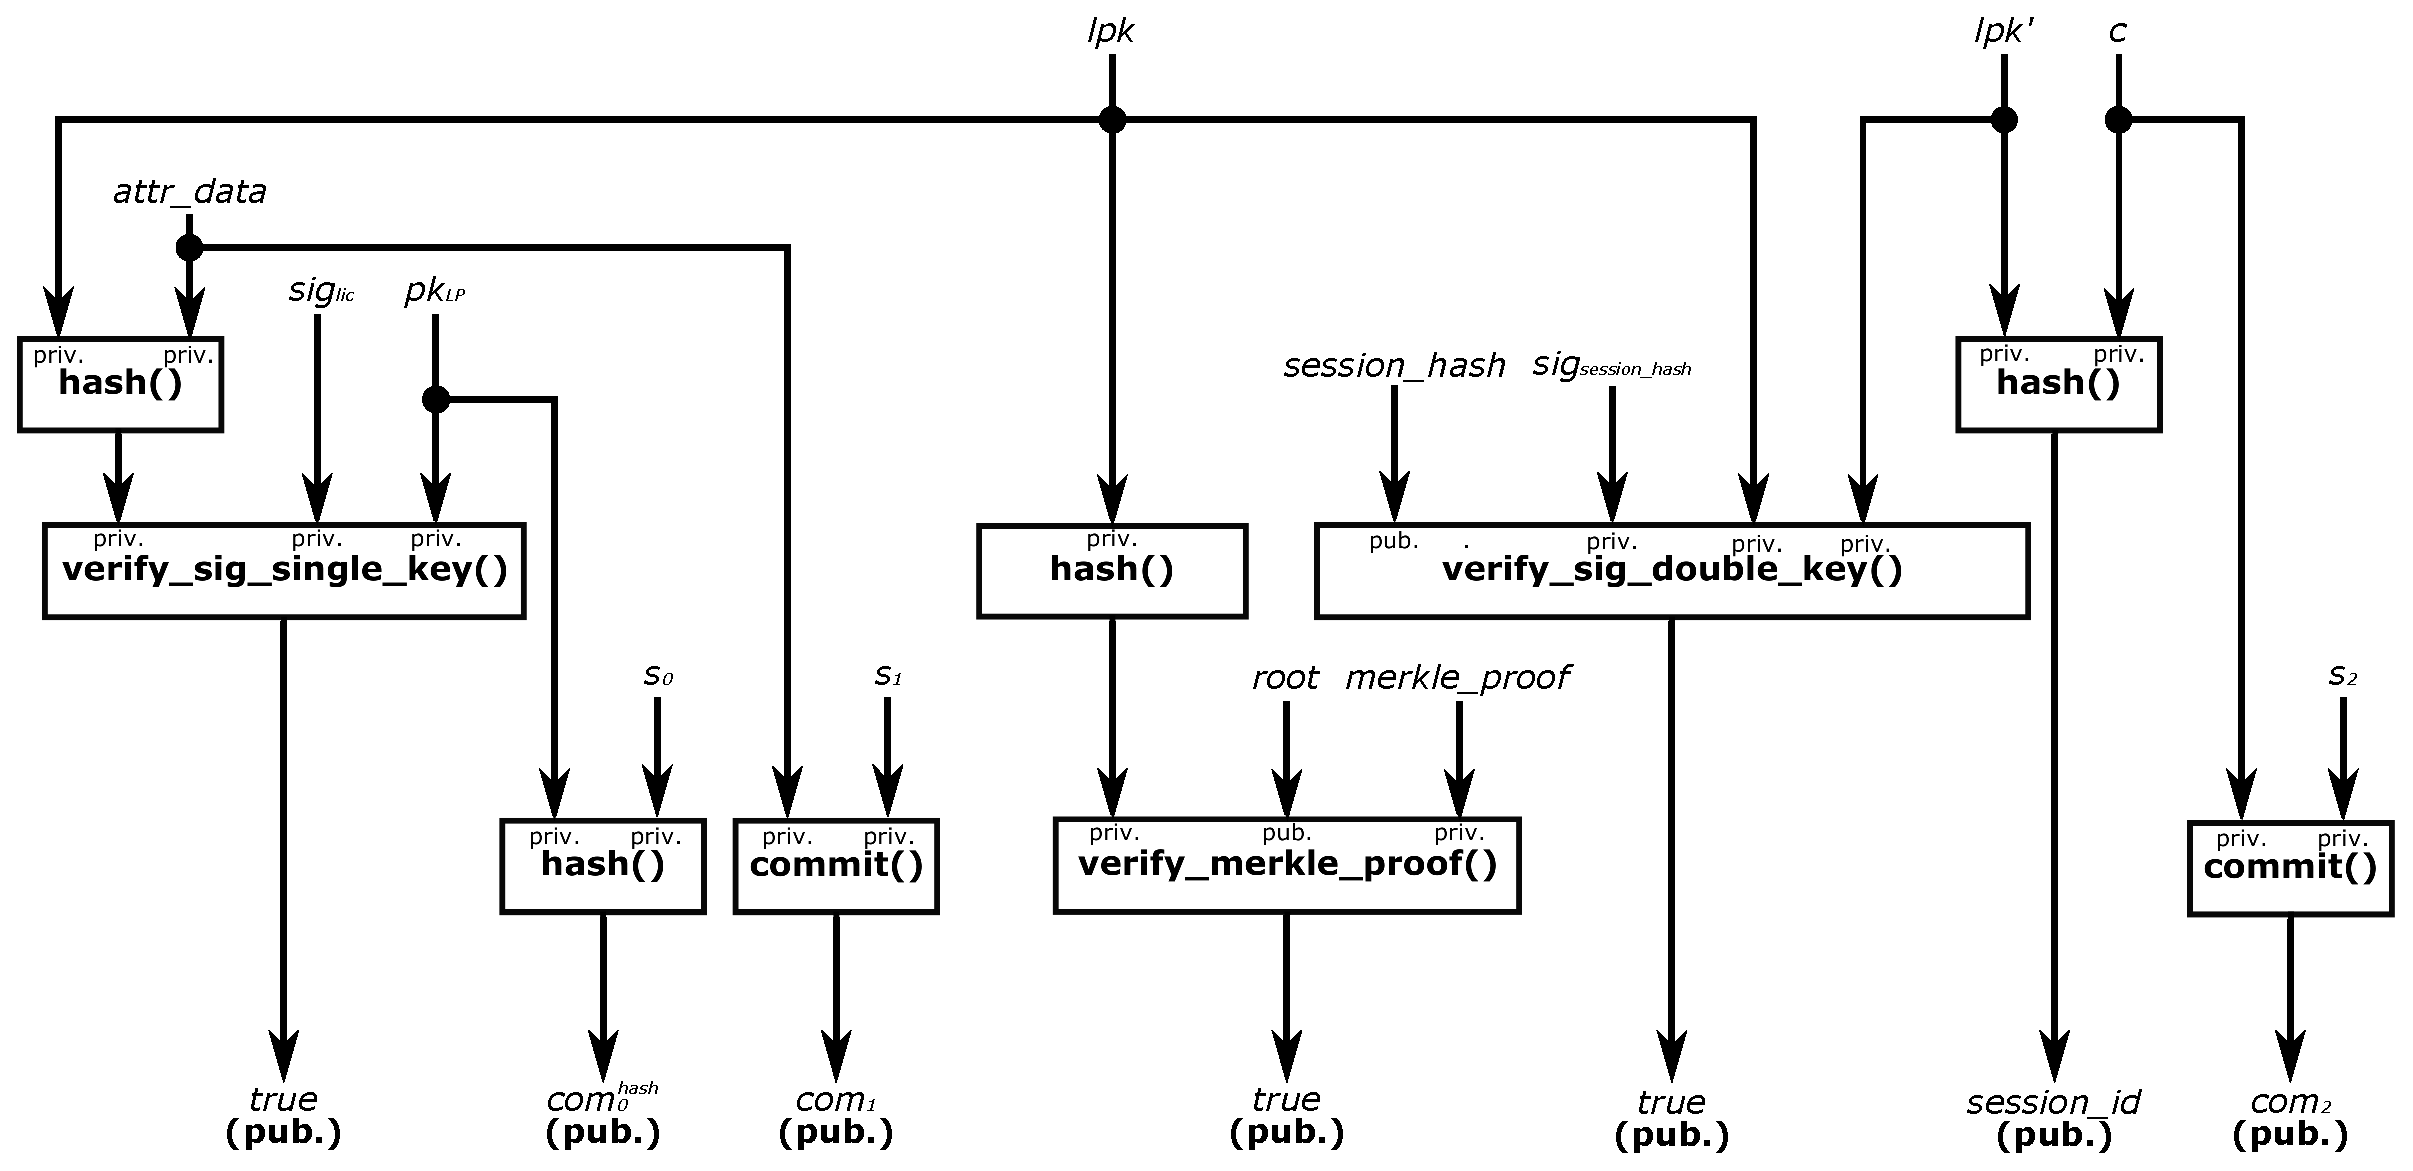
\includegraphics[width=460pt,draft=false]{images/circuit_prove_nft.eps}}
%	\caption{Arithmetic circuit for proving a license's ownership.}
%	\label{fig:circuit_prove_nft}
%\end{figure}

\mbi{The following paragraph needs a bit more elaboration on the different use cases. Maybe discuss this in the first section of the document?}

Furthermore, the SP might want to prevent the user from using the license more than once (e.g. this is a single-use license, like entering a concert). 
This is done through the computation of $\sessionid$. The deployment of this part of the circuit has two different possibilities:

\begin{itemize}
	\item By setting $c = 0$ (or directly remove this input from the circuit), the license can be used only once.
	\item If the SP requests the user to set a custom value for $c$ (e.g. the date of an event), the license can be reused only under certain conditions.
\end{itemize}

